



\section{Day ahead and real time energy prices}




\section{Characteristics of energy markets}

Ideas: 

\begin{itemize}
	\item Show electricity price variation for market over a 3 year period (Weron, pg 33)
	\item Show autocorrelation function over extended (same) time period
	\item Show periodogram over extended time period
\end{itemize}

%
%Active research topics in this field include electricity cost reduction in data centers \cite{guler2013cutting, le2011reducing}. A comparison of different approaches considering spatial and temporal energy price changes and the contribution of the outside temperature to the resulting cooling effort and expense is outlined in \cite{guler2013cutting}. In \cite{le2011reducing} a set of homogenous data centers is simulated where the focus lies on the effects of changing workloads and migrations on the cooling infrastructure and on intelligent scheduling to reduce energy consumption and energy costs, respectively. 
%
%The authors in \cite{lucanin2013take} propose a green cloud approach using real time electricity prices where the duration and time of price peaks are estimated and VMs are paused during these times to reduce energy costs and save energy. Customers may choose between ``green'' and normal instances, taking into account some loss of availability for a reduced price. 
%
%
%
%In \cite{rao2010minimizing} a cloud consisting of several Internet Data Centers (IDC) is examined with regard to cost optimization which is done by intelligently assigning workload to data centers based on current energy prices. Two of these data centers in the scenario are connected to deregulated wholesale energy markets whereas the other one is connected to a regulated utility region charged by a fixed pricing scheme. Since price change differences in deregulated energy markets can be considerable energy cost reductions may be achieved by assigning workload based on changing energy prices.  %For the purpose of the simulation five front-end Web portal servers process a total workload of about $10^5$ requests per second. 
%
%In this paper the approaches of optimal and average workload assignments are visually and formally compared to gain insights into the total electricity cost reduction. The optimal workload assignment is calculated with respect to workload and delay constraints that are considered in a minimum cost flow problem based on a linear programming model. Thus the goal is to minimize costs without compromising quality of service constraints. 
%%The proposed cost reductions amount up to 30 percent for a single hour test within the given time range. 
%%The results measured at two timestamps at a specific day seem promising, since total cost reductions could be achieved by 30\% and 17\% respectively. 
%
%The differences compared to this work is that in \cite{rao2010minimizing} they do not consider longer running jobs as used in scientific calculations or large optimization problems that may take several hours to complete. Thus the impact of migrations is not examined in this scenario. In addition the possibility of energy price forecasting is not considered which may result in even greater energy cost reductions. 
%
%Another study on cost reductions in Internet Data Centers has been done where different aspects of cost reductions including cost prediction schemes have been considered \cite{de2013study}. Since up to 15\% of total capital investment is spend on energy related costs 
%%(paper references \cite{greenberg2008cost} - old, from 2009!!) 
%a special effort is invested to reduce the amount of energy costs through cost aware operations. %(TODO: Move to introduction?)
%
%In this paper cost optimization is seen as an assignment problem where an overall cost function is minimized through intelligent workload allocation. During the investigation different variables and their impact on resulting energy costs are considered which are price volatility, price predictions including variable prediction errors, time lag between locations and reconfiguration delays. 
%
%Similar to this work the simulation is run with the same set of fixed parameters to evaluate the impact of the various scenarios. It is observed that prediction errors greatly impact workload allocation where cost penalties due to non-optimal assignments increase quadratically with an increase of forecast errors \cite{de2013study}. Also with increasing number of locations the minimum cost of optimal assignments can be greatly reduced. Greater price volatility is beneficial as well since then price aware assignments will have greater impacts. 
%
%A comprehensive study on cost reductions and energy market characteristics in an environment where data centers are placed within the reach of different energy markets is presented at \cite{qureshi2009cutting}. Based on geotemporal variations of energy prices the maximum cost reductions under different scenarios are evaluated. Energy expenses are estimated for various large scale companies like Google and Yahoo to state the actual savings and the amount of reductions in energy costs that would be possible. 
%They also discuss the impact of considering bandwith constraints and maximum client server distances on cost reductions. 
%
%Interestingly enough long term seasonalities in the energy price data has been discovered that spanned multiple energy markets. This is an important fact when training forecasting models since predictions can become a lot more accurate. An important fact that was revealed about energy markets was that data from different energy markets was much less correlated than data from the same area. Thus to take full advantage of energy price differences data centers located at different energy markets should be combined \cite{qureshi2009cutting}. 
%
%With different state of the art energy models and simulation constraints a summary of possible cost reduction schemes was presented. However no migration or forecasting of energy price data has been done which could further improve scenarios with longer running jobs. In addition these cost reductions are only valid under specific assumptions that large cloud providers would need to implement such as connection to wholesale energy markets and reasonable server energy elasticity. 
%
%
%
%
%\subsection{Server power management}
%
%A well known problem in power management is how to accurately and efficiently model a server's power consumption over time. At \cite{horvath2008multi} Horvath et al.~exploit dynamic voltage scaling (DVS) and multiple sleep states to reduce power consumption of a server cluster of about 23\% without significantly impacting performance. They propose that CPU utilization and frequency are the variables that have the most significant impact on the power consumption of a machine. This assumption is also used in other studies, e.g.~\cite{rao2010minimizing, hammadi2014survey, kliazovich2012greencloud}. 


See folders "`Electricity pricing"' and "`power markets"'


\begin{figure}[htbp]
	\centering
		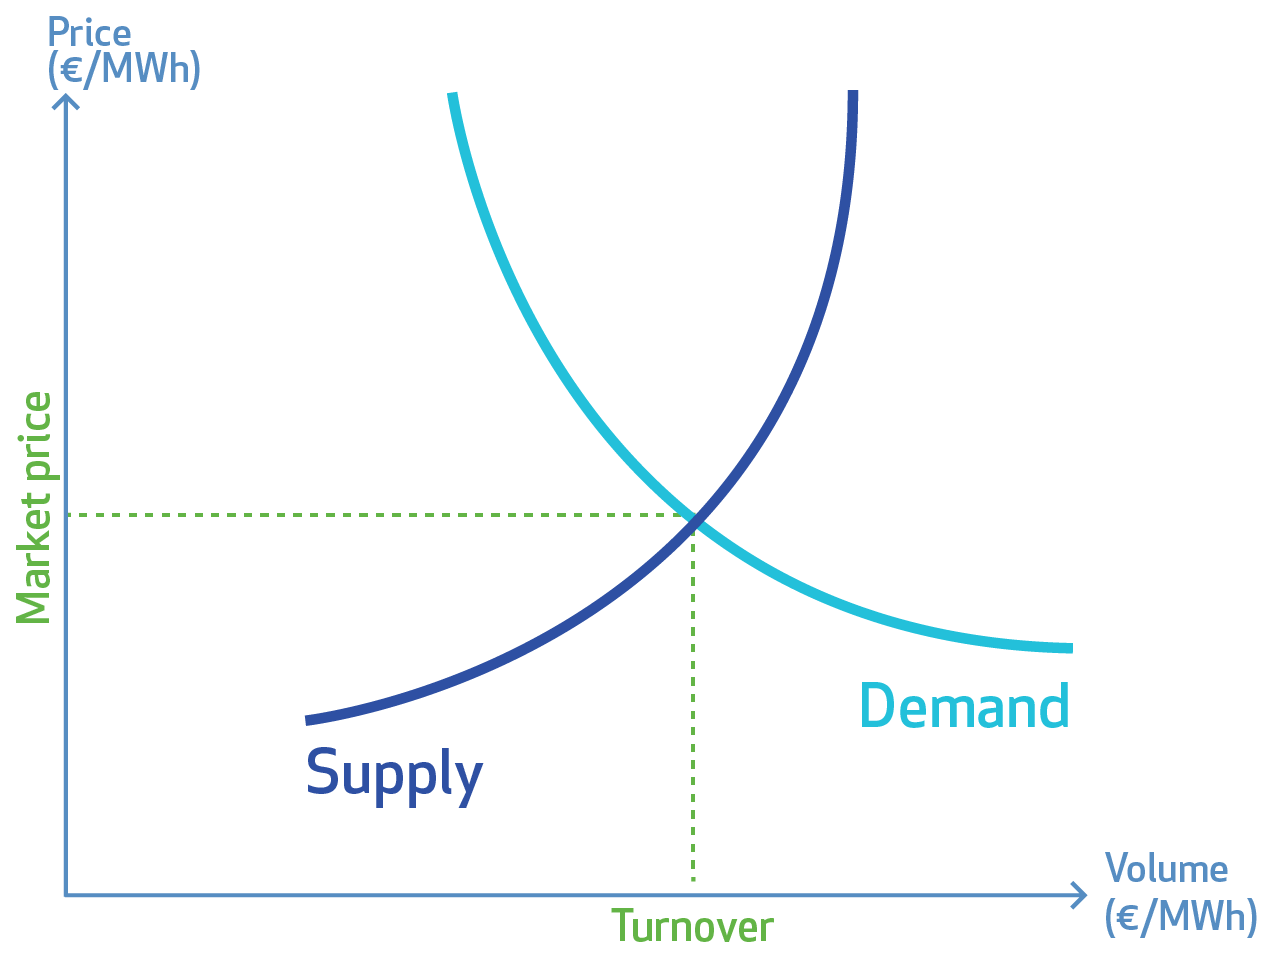
\includegraphics[width=0.5\textwidth]{figures/data_analysis/DA_supply_demand.png}
	\caption{Intersection between supply and demand \cite{nord2014supply}}
	\label{fig:DA_supply_demand}
\end{figure}



In this section different studies of power market characteristics are presented to distinguish features that may be used in building forecasting models. 

\subsection{Stable Modeling of different European Power Markets}

In this paper different European power markets have been investigated to reveal major differences in energy price behaviour \cite{mugele2005stable}. The EEX, Nord Pool Spot and Polish power markets have been evaluated whereby the markets are responsible for the Mid-Europe, Northern Europe and Polish regions respectively. 

As in general electricity prices depend on energy demand \cite{weron2005forecasting} which changes due to climate conditions (temperature and number of daylight hours) electricity prices exhibit a seasonal component as well (Figure \ref{fig:seasonal_behaviour_of_eex_prices}). 

\begin{figure}[htbp]
	\centering
		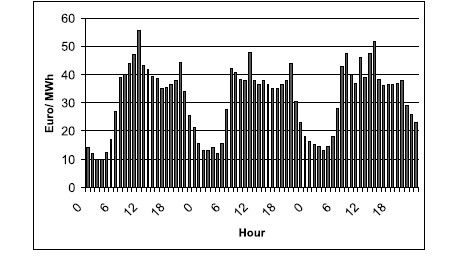
\includegraphics{figures/state_of_the_art/seasonal_behaviour_of_eex_prices.PNG}
	\caption{EEX - hourly spot prices \cite{mugele2005stable}}
	\label{fig:seasonal_behaviour_of_eex_prices}
\end{figure}

The main differences between electricity power markets and other financial markets are price volatility, mean reversion and price jumps or "`spikes"'. Volatility is high as generated electricity cannot be stored but has to be delivered at once which might lead to high prices on transmission congestion or surges in demand. It's impact can be reduced by applying logarithmic transformations of input data \cite{weron2005forecasting}. 

Energy prices experience strong mean reversion which denotes the characteristic that prices return to their mean levels after an increase in prices. In addition price spikes may appear where prices can increase tenfold from one hour to the next. To mitigate these spikes they may be averaged out in a data preprocessing step. 

Even though price seasonality and trend seem to be stable over a short time range (Figure \ref{fig:seasonal_behaviour_of_eex_prices}) they can show significant fluctuations over a longer time range. In \cite{mugele2005stable} data related to each examined energy market was fitted to a stable Paretian distribution as well as a normal distribution. The result showed that mature markets as EEX or Nord Pool Spot exhibit high volatility, heavy tails, high kurtosis and asymmetrics in the energy price data which was best modeled by the Paretian distribution. In contrast the Gielda Energii SA market in Poland shows a much more stable energy price behavior which can be modeled by a Gaussian distribution. 

The variation in energy price levels for the two power markets EEX and Nord Pool Spot are shown in Figures \ref{fig:EEX_levels} and \ref{fig:NordPool_levels}.

\begin{figure}[!htbp]
  \centering
  \begin{minipage}[b]{0.4\textwidth}
    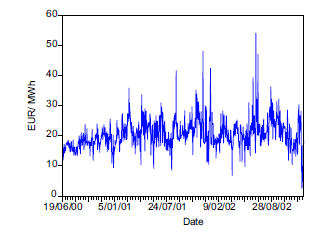
\includegraphics[width=\textwidth]{figures/state_of_the_art/EEX_levels.PNG}
    \caption{EEX levels \cite{mugele2005stable}}
		\label{fig:EEX_levels}
  \end{minipage}
  \hfill
  \begin{minipage}[b]{0.4\textwidth}
    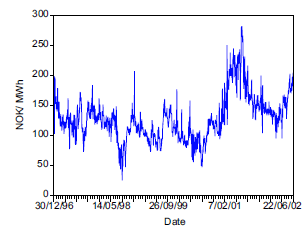
\includegraphics[width=\textwidth]{figures/state_of_the_art/NordPool_levels.PNG}
    \caption{Nord Pool levels \cite{mugele2005stable}}
		\label{fig:NordPool_levels}
  \end{minipage}
\end{figure}

This shows that it is important to investigate energy price characteristics from power markets to accurately model market prices. 



%
%\subsection{Electricity markets and pricing}
%
%In wholesale energy markets different pricing and bidding models can be used. Currently the two most common price evaluation strategies are day-ahead and real-time pricing strategies. 
%
%\subsubsection{Bidding strategies}
%
%In \cite{tierney2008uniform} two different bidding strategies are discussed, uniform pricing and pay-as-bid auctions. In the uniform pricing model the market clearing price is determined by collecting the marginal prices from all suppliers and taking the maximum price from this collection. Conversely, in pay-as-bid auctions a supplier gets paid based on its actual bid. 
%The second approach may seem beneficial from the customer's point of view since suppliers may set individual prices which enables competition within the market. 
%However studies show that in this pricing scheme suppliers set their prices at the maximum possible level to be comparable to other suppliers and keep their customers. On the other hand the uniform pricing model provides a uniform clearing price which is valid for all participants in the market and customers may trust that suppliers set prices to just satisfy their needs. 


\section{Energy price case study}



